%% The beamer class for presentation.
% \title[<Short Title>]{<Full Title>}
% \author[<Short Name>]{<Full Name> \\ <gmail>}
% 
% In beamer, a presentation consists of a series of frames. Each frame in turn may consist of several slides.
% We can add also:
%\tableofcontents
%\section
%\subsection
%
%\begin{lstlisting}
%\end{lstlisting}
%
% Verbatim: আক্ষরিকভাবে। যেভাবে আছে ঠিক সেভাবেই।
%
%\begin{block}{Write something here}
%\end{block}
%
%\begin{definition}
%\end{definition}
%
%\alert{}
%
%\begin{verbatim}
%\end{verbatim}
%
%\begin{proof}
%\end{proof}


\documentclass[9 pt]{beamer}

\usepackage
{
	listings, % Program Code Listing.
	authblk, % Redefines \author command. Permits footnote type affiliation.
	anyfontsize,
	graphicx,
	transparent % Control image/text transparency. OR, make a transparent photo from photoshop.
}

\title[Graphics Tutorial]{C Graphics Function}
\subtitle{Brief Descriptions for C Graphics}
\author[S. I. Kiron]
{
	Sofiullah Iqbal Kiron \\
	\href{mailto:sofiul.k.1023@gmail.com}{sofiul.k.1023@gmail.com}
}
\date[Wednesday]{30 Dec, 2020}
\institute[BSMRSTU]{Bangobandhu Sheikh Mujibur Rahman Science and Technology University}
\affil{Department of CSE}

\lstset
{
 language = C++,
 backgroundcolor = \color{white},
 basicstyle = \footnotesize\ttfamily,
 keywordstyle = \color{blue},
 commentstyle = \color{green!80}\tiny,
 showstringspaces = false,
 stringstyle = \color{red},
 captionpos = b
}


%\usetheme[progressbar=foot, numbering=fraction, background=light]{metropolis}
\usetheme{Madrid}
\useinnertheme{rounded}
\usecolortheme{default}

\begin{document}

{ % Local background surrendered in a pair of curly brace. Wanna add globally? put command at preamble.
\usebackgroundtemplate{\transparent{0.4}{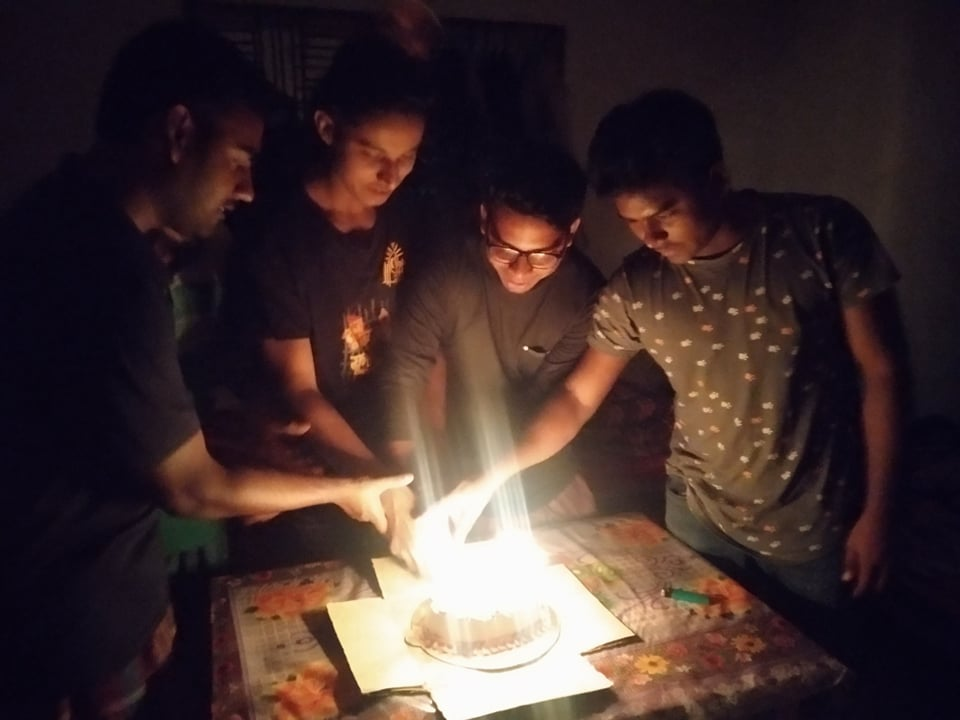
\includegraphics[width=\paperwidth, height=\paperheight]{Picture/TitlePage Background Original.jpg}}}
\frame
{
	\titlepage
}
}

\begin{frame}[fragile]
	\frametitle{graphics.h function}
	\framesubtitle{putpixel()}
	\pause
	\alert{Syntax:}
\begin{lstlisting}
	void putpixel(int x, int y, enum color);
\end{lstlisting}
\pause
This function will put a pixel at the given coordinates by the color specified.\pause \\
Now, take a color form the \emph{enum} list.
\begin{lstlisting}
	enum colors { BLACK, BLUE, GREEN, CYAN, RED, MAGENTA,
	BROWN, LIGHTGRAY, DARKGRAY, LIGHTBLUE, LIGHTGREEN,
	LIGHTCYAN, LIGHTRED, LIGHTMAGENTA, YELLOW, WHITE };
\end{lstlisting}
{\texttransparent{0.2}{Hello}}
\end{frame}

\begin{frame}[fragile]
\frametitle{The delay() function}
\framesubtitle{No subtitle}
\pause
\alert{Syntax:}
\begin{lstlisting}
	void delay(int milisecond);
\end{lstlisting}
\pause
\begin{block}{Description}
Delay/Pause program for miliseconds. (1000/1k miliseconds = 1 second)
\end{block}
\end{frame}

\begin{frame}[fragile]
\frametitle{Draw a line using putpixel function: Animated}
\framesubtitle{No subtitle}
\pause
\begin{lstlisting}[caption=Animated Line, basicstyle=\small]
void drawAnimatedLine()
{
    int start, end;
    printf("Starting point: ");
    scanf("%d", &start);
    printf("Ending point: ");
    scanf("%d", &end);
    while (start <= end)
    {
        putpixel(start++, 250, GREEN);
        delay(5);
    }
}
\end{lstlisting}
\end{frame}

\begin{frame}[fragile]
\frametitle{Rectangle Anime}
\framesubtitle{Drawing an rectangle by putpixel() and delay() function}
\pause
\begin{lstlisting}[basicstyle=\tiny, frameround=fttt, frame=trBL, numbers=left]
void drawAnimatedRectangleFromMid() {
    int midX, midY, totalHeight, totalWidth, i, j;

    printf("Mid point-X: "); scanf("%d", &midX);
    printf("Mid point-Y: "); scanf("%d", &midY);
    printf("Total Width: "); scanf("%d", &totalWidth);
    printf("Total Height: "); scanf("%d", &totalHeight);

    // Drawing up line.
    i = midX, j = midX;
    while (i >= midX - totalWidth / 2) {
        putpixel(i--, midY, GREEN); putpixel(j++, midY, GREEN);
        delay(9);
    }

    // Drawing side lines.
    i = midY, j = midY;
    while (i <= midY + totalHeight) {
        putpixel(midX - totalWidth / 2, i++, GREEN); putpixel(midX + totalWidth / 2, j++, GREEN);
        delay(9);
    }

    // Drawing bottom line.
    i = midX - totalWidth / 2, j = midX + totalWidth / 2;
    while (i <= midX) {
        putpixel(i++, midY + totalHeight, GREEN); putpixel(j--, midY + totalHeight, GREEN);
        delay(9);
    }

    /* Over */
}
\end{lstlisting}
\end{frame}

\begin{frame}[fragile]
\frametitle{graphics.h function}
\framesubtitle{line()}
\pause
\alert{Syntax:}
\begin{lstlisting}
void line(int x1, int y1, int x2, int y2);
\end{lstlisting}
\pause
\begin{block}{Description}
Will draw a straight line from $(x1, y1)$ to $(x2, y2)$.
\end{block}
\end{frame}

\begin{frame}[fragile]
\frametitle{graphics.h function}
\framesubtitle{setcolor()}
\pause
\alert{Syntax:}
\begin{lstlisting}
void setcolor(enum color);
\end{lstlisting}
\pause
\begin{block}{Description}
After this statement, all graphical elements will be colored as defined in the function.
\end{block}
\end{frame}

\begin{frame}[fragile]
\frametitle{graphics.h function}
\framesubtitle{rectangle()}
\pause
\alert{Syntax:}
\begin{lstlisting}
void rectangle(int left, int top, int right, int bottom);
\end{lstlisting}
\pause
\begin{block}{Description}
Give the coordinate of top-left(left, top) and bottom-right(right, bottom) corner. Then a rectangle will be created.
\end{block}
\end{frame}

\begin{frame}[fragile]
\frametitle{Draw Rectangle Shape Bar}
\framesubtitle{Animated Rectangle Bar}
\pause
\begin{lstlisting}[caption=Filling a rectangle with rectangle, basicstyle=\footnotesize, numbers=left]
void barTypeRectangleAnimated()
{
    int left, top, right, bottom;
    printf("Left: ");
    scanf("%d", &left);
    printf("Top: ");
    scanf("%d", &top);
    printf("Right: ");
    scanf("%d", &right);
    printf("Bottom: ");
    scanf("%d", &bottom);

    while (left < right - 5 && top < bottom - 5)
    {
        rectangle(left++, top++, right--, bottom--);
        delay(9);
    }
}
\end{lstlisting}
\end{frame}

\begin{frame}[fragile]
\frametitle{Any Font Size}
\framesubtitle{Still not arrived!}
\begin{block}{Description}
You can give any size of a font as you want by using \textit{anyfontsize} package. And then the command.
\end{block}
\end{frame}

\end{document}
